% !TeX root = ../main.tex
% !TEX spellcheck = en_GB

\chapter{Architecture}
\label{sec:Architecture}
This section describes the overall system architecture, the chosen platforms for development and how the different subsystems communicate with each other.

\begin{figure}[H]
	\centering
	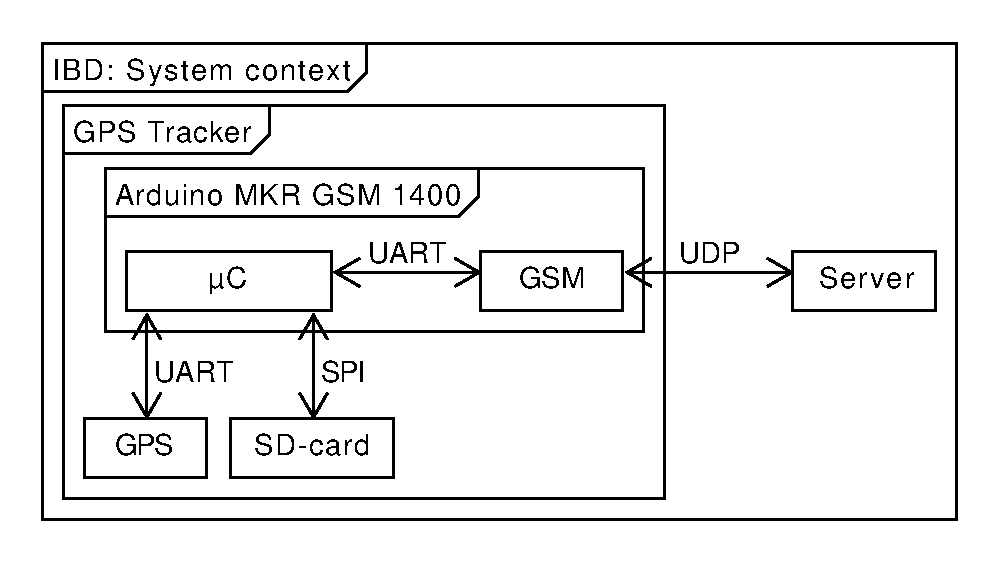
\includegraphics[width=0.7\linewidth]{gfx/Design/Overall_IBD.pdf}
	\caption{Overall IBD, including types of connection.}
	\label{fig:IBD:overall}
\end{figure}

\section{Choice of components}
The physical entities necessary to solve the tasks of the blocks identified in \cref{fig:IBD:overall} are as follows:

\paragraph{Controller and Data transfer} can be performed by a single module. The \MKR which includes a \SAMD ARM µC and a u-blox SARA-U201-03B-00 High Speed Packet Access (HSPA) with 2G fallback module for internet access\cite{MKRGSM1400}.
They communicate using one of the two UARTs available on the \SAMD ARM µC.
The \SAMD ARM µC uses \SI{< 15}{\milli\ampere} while running \cite[p.~791-794]{SAMD21}.
The SARA-U201 uses a maximum of \SI{1.9}{\ampere} when transferring data \cite[p.~26]{SARAU201} and less than \SI{1}{\milli\ampere} when in power-saving mode. Alternatively the known Arduino MEGA2560 with an external GSM module could be used, but this has been opted against in favour of using an integrated low power module.

\paragraph{Locator} has to be able to locate itself globally. This is solved using the GNSS module, u-blox NEO-7M-0-000, from Embedded Stock.
The module is able to use GPS (with SBAS and QZSS) and GLONASS, allowing for global positioning.
It also uses a maximum of \SI{67}{\milli\ampere} \cite[p.~17]{NEO7_Data} and is the low power version from the NEO-7 series.
The breakout-board exposes the UART connection, which can be used to communicate with the controller.

\paragraph{Memory} has to be non-volatile and able to store at least 1440 locations.
This is accomplished using a SD-card with \SI{2}{\giga\byte} of memory, allowing for each location to be up to \SI{1.39}{\mega\byte}.
The connection to the \SDsock SD-card breakout board\cite{Ciseco} is SPI which is directly available on the \MKR module.

\section{Communication}
With the chosen components, the interfaces between them can be identified, as shown in \cref{fig:IBD:overall}.
The communication between the \SAMD and the \SARA module are presoldered to UART.
The breakout-board for the \GPS exposes UART ports and the SD-card breakout-board exposes SPI ports.
Connection to the server is chosen to be UDP with an acknowledge from the server.

\subsection{\MKR and \GPS}
The \GPS UART uses the frame 8N1, with a baud rate of \num{4800}, \num{9600}, \num{19200}, \num{38400}, \num{57600} or \num{115200}.
For easy debugging, the \num{9600} baud rate is chosen.

\subsubsection{Protocol}
\label{sec:UBXprot}
The chosen GPS module is able to communicate using NMEA, UBX or RTCM protocol \cite{NEO7_proto}.
It has been chosen to communicate using the UBX protocol, as it, asides from the GPS location data, can be used to set up the modules internal workings, such as power save mode.

\Cref{fig:UBX} shows the UBX protocol.
The sync chars are static and the CLASS and ID define the function which the \GPS is meant to perform.
The checksum is calculated using the CLASS, ID, length and payload bytes, as described in \cite[p.~74]{NEO7_proto}.
Two types of responses from the \GPS.
If the command is a setup command, the \GPS answers with ACK or NACK \cite[p.~80]{NEO7_proto}.
Any other command will respond with the answer described in the protocol.
See \cite[p.~73-183]{NEO7_proto} for the full protocol, or below for an example.

\begin{figure}
	\centering
	\includegraphics[page=86, width=\textwidth,  clip, trim={2cm, 14cm, 2cm, 10cm}]{Appendix/Datasheets/u-blox7-V14_ReceiverDescrProtSpec_(GPS-G7-SW-12001)_Public.pdf}
	\caption{Overview of the UBX protocol \cite[p.~73]{NEO7_proto}.}
	\label{fig:UBX}
\end{figure}

The most used UBX command is UBX-NAV-PVT \cite[p.~160]{NEO7_proto}, which returns the location of the \GPS.
The communication is shown in \cref{tab:UBXex}.
Answers are available from the later performed tests, but can be seen in \cref{app:GPSmodtest} and \cref{app:GPSinttest}.

\begin{table}
	\centering
	\begin{tabularx}{\textwidth}{l l X}
		\toprule
		& \textbf{Command} & \textbf{Description} \\
		\midrule
		Sync Char 1 & 0xB5 & Hex value for the ascii char µ. \\
		Sync Char 2 & 0x62 & Hex value for the ascii char b. \\
		CLASS & 0x01 & Navigation Results. \\
		ID & 0x07 &  Navigation Position Velocity Time Solution. \\
		Length & 0x0000 & Length of payload. \\
		Payload & NONE & Here no payload is needed, as the CLASS and ID tells the \GPS what to return. \\
		CK\_A & 0x08 & Checksum part A. \\
		CK\_B & 0x19 & Cheksum part B. \\
		\bottomrule
	\end{tabularx}
	\caption{Example communication using the UBX protocol.}
	\label{tab:UBXex}
\end{table}

\subsection{\SAMD and \SARA}
As is standard with GSM modules, the \SARA employs a AT command interface through the UART. This means that commands and data to and from the module is in ascii, and that commands is started by "+AT" and end with <CR><LF>. 

The implementation and design of communications between \SAMD and \SARA will follow specification laid out in PDF\fxnote{Ref u-blox-CEL\_ATCommands\_(UBX-13002752).pdf}. 

In general each communication will follow a given flow, the controller starts by sending an AT command:

\mint{bash}{AT+CREG?\r\n}

Responding to each message the GSM module responds with the command it read:

\mint{bash}{AT+CREG?\r}

Following command confirmation, if it is a recognised command, the GSM will potentially send a respond message with status. This responds always starts with a '+' symbol. 

\mint{bash}{AT+CREG: 0,1\r}

Finally a last message will be send, with the result code of the command. This will either be "OK" or "ERROR". If the command was not recognised the result will always be "ERROR".

\mint{bash}{OK\r\n}

\fxnote{Allocation Diagram?}


\FloatBarrier